\documentclass[10pt]{article}
\usepackage[margin=0.78in]{geometry}
\usepackage{amsmath,amssymb,longtable,booktabs,graphicx,xcolor}
\usepackage{xurl,needspace}
\usepackage[colorlinks=true,breaklinks=true,urlcolor=blue]{hyperref}
\emergencystretch=2em
\setlength{\parindent}{0pt}
\setlength{\parskip}{5pt}
\title{Weak elliptic-curve families: classification,\\ recognition and evidence}
\author{Research catalogue and model index}
\date{10 October 2026}
\begin{document}
\maketitle
The catalogue contains 21 family or condition entries and 814 exact synthetic model records. It organizes published subgroup reductions and covering families alongside proved class support, verified geometry and structural leads. Every record states its field, subgroup, recognition and construction scope.

\section{Classification contract}
A model condition, class-support theorem, source construction and subgroup cost comparison are distinct evidence levels. A covering witness establishes geometry; a subgroup condition and a verified cost are needed for a selected-group comparison. Necessary filters and structural signals retain their own labels.

The model index contains 277 postselected $p=7$ route/conversion/control models, 25 larger-degree constructed-control models, and 512 original independent large-field sources. The complete $p=7$ torus images and ordinary $t\equiv2\pmod4$ trace oracle provide exact local labels. Large-field class labels remain unresolved after the recorded bounded searches. Inventory counts are not population density estimates.

\begin{figure}[ht]\centering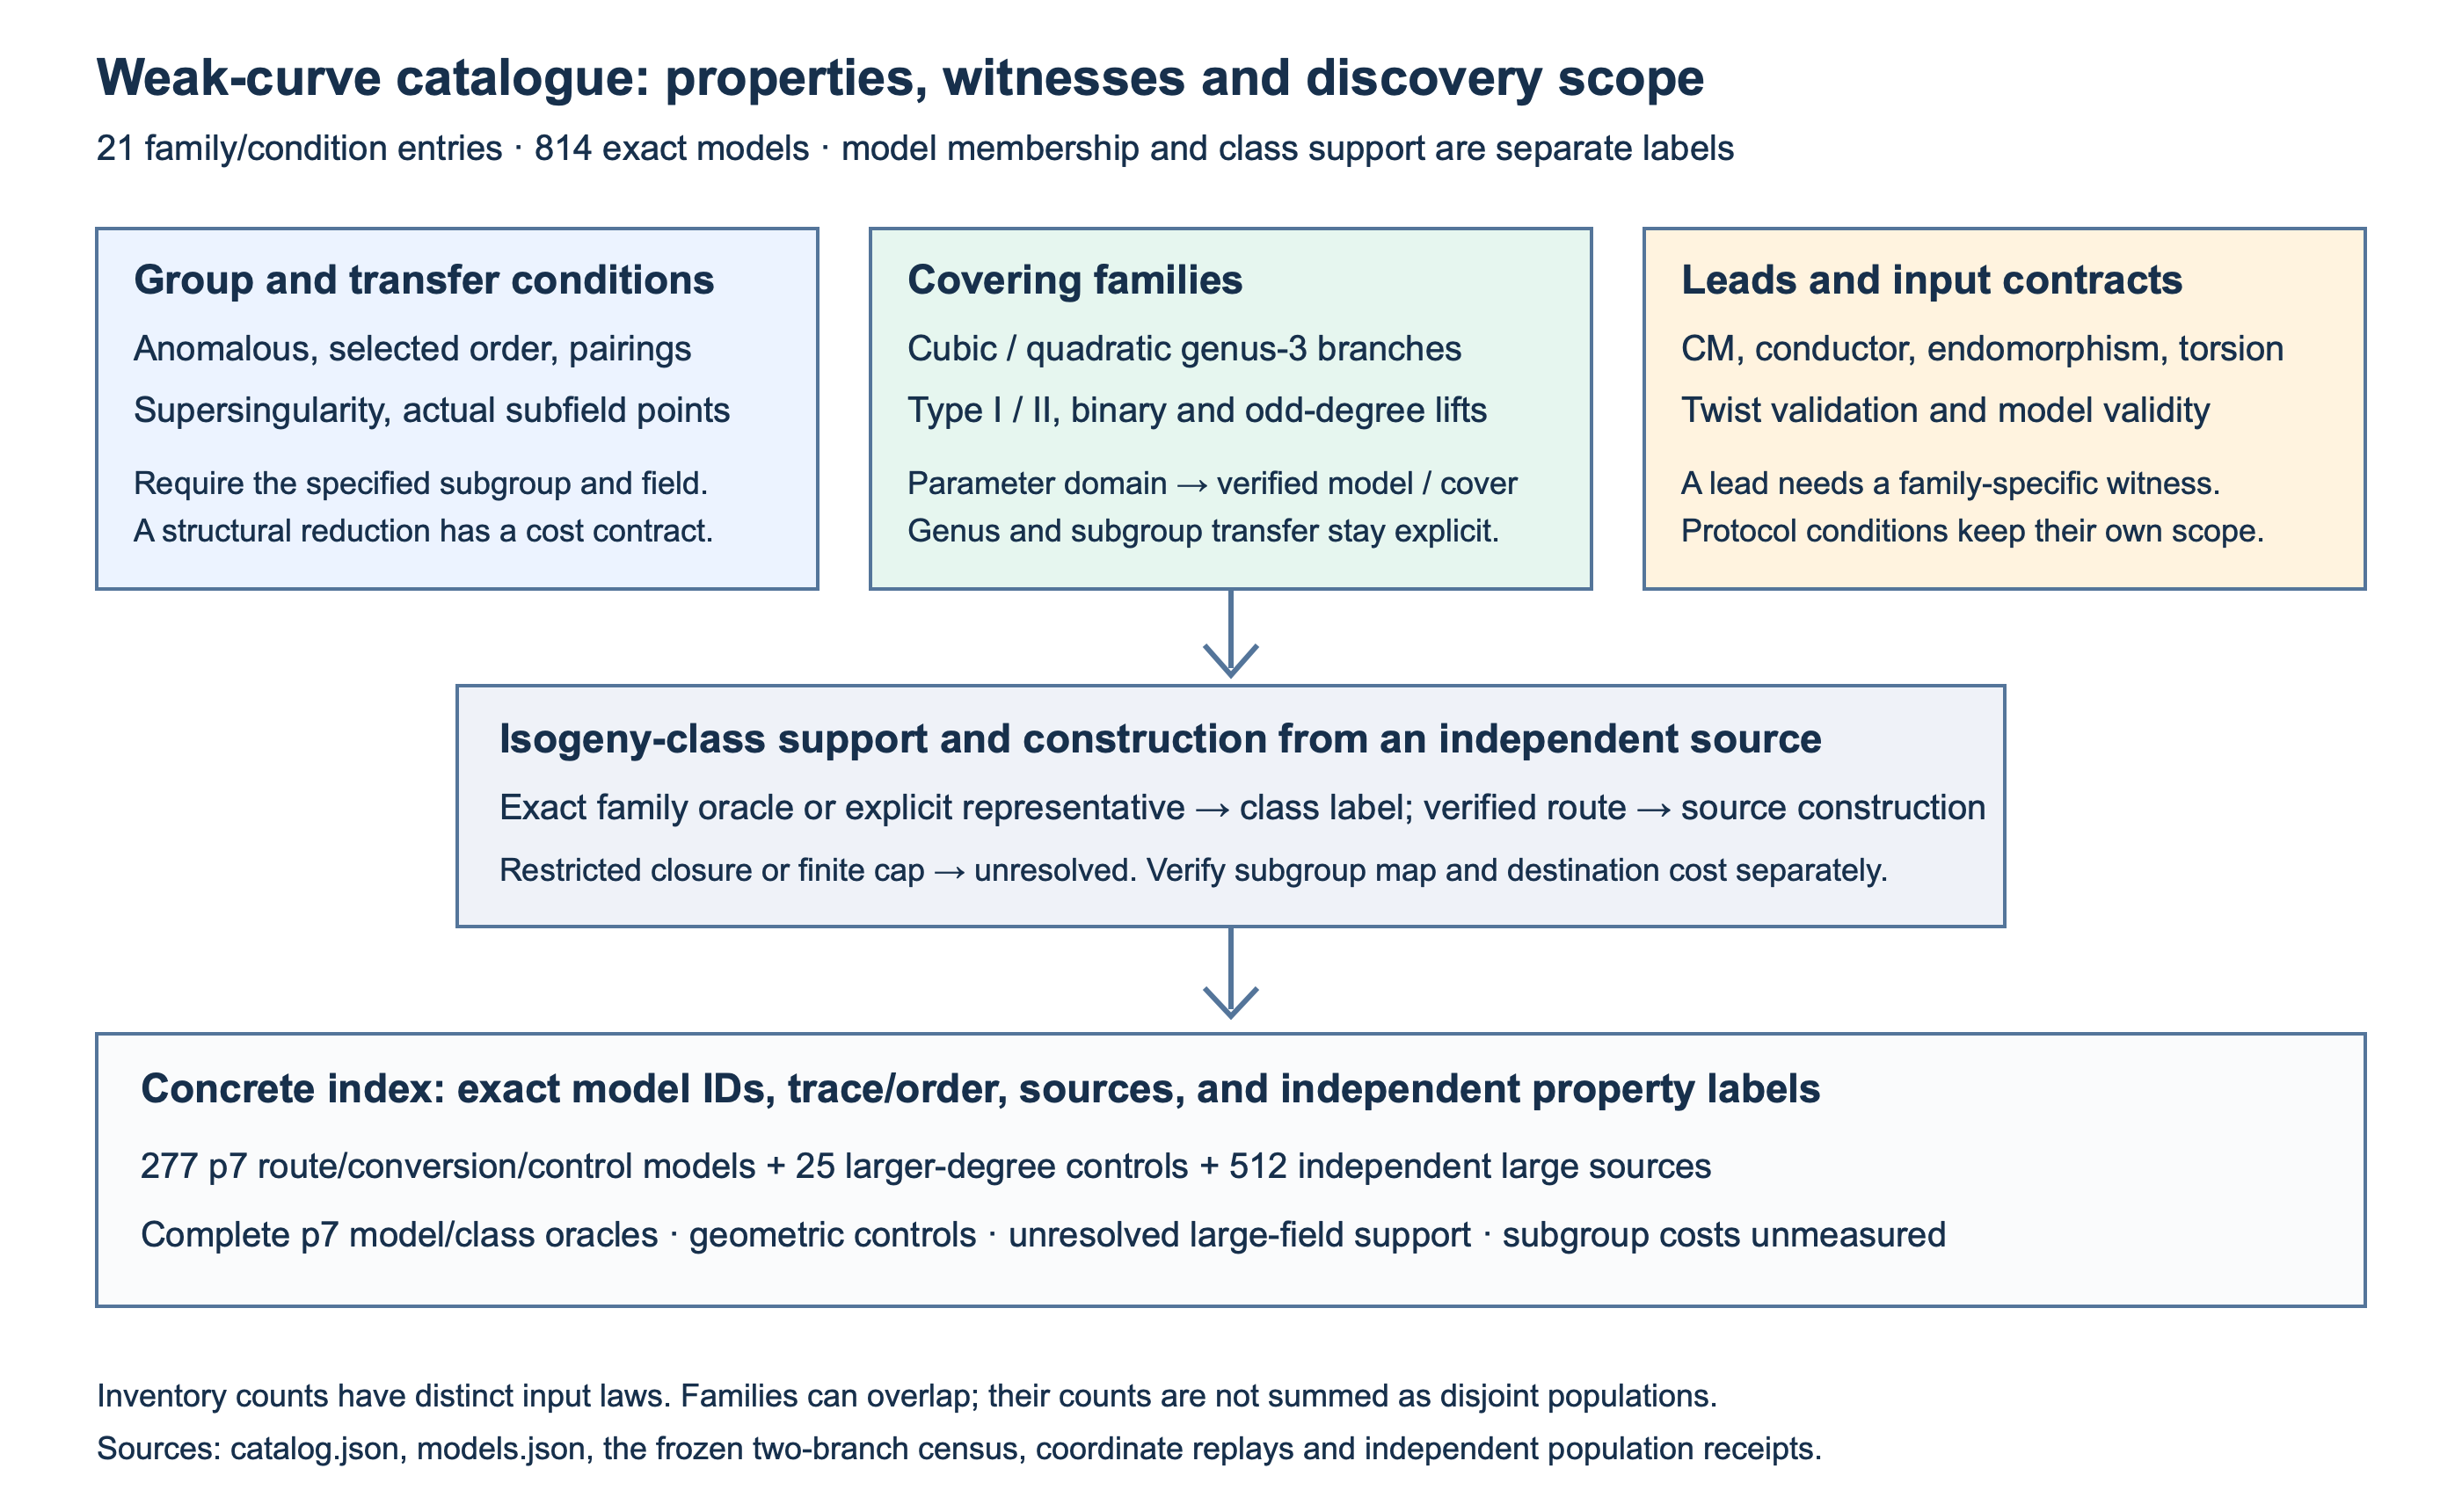
\includegraphics[width=\linewidth]{classification.png}\caption{Classification proceeds from a scoped property to its appropriate witness and cost contract. Conditional links retain their hypotheses.}\end{figure}
\section{Catalogue entries}
The published families retain their original attribution. Momose--Chao classify Type I/II coverings and their hyperelliptic subcases; Joux--Vitse develop cover/decomposition index calculus. The attached ISO-1 contribution is the exact ordinary isogeny-class support criterion for the two hyperelliptic branches, complete finite class oracles, and independently replayed source constructions. This catalogue unifies the identity and evidence records across mechanisms.

\Needspace{8\baselineskip}\subsection{Anomalous prime-field curves}
\texttt{WCF1:anomalous-prime}\quad subgroup reduction / published reduction.\par
\textbf{Domain.} Nonsingular E over F\_p, p prime, selected group E(F\_p).\par
\textbf{Recognition.} Exact N = p, equivalently trace t = 1. Near equality is a different condition.\par
\textbf{Find members.} For a fixed prime, a certified trace-one enumeration or trace-prescribed construction gives members. Exact counting certifies the predicate.\par
\textbf{Completeness.} All nonsingular prime-field models whose certified trace equals one; equivalent models require identity-aware deduplication.\par
\textbf{Subgroup and cost.} Specify the characteristic-order group and the hypotheses of the cited p-adic reduction. Retain construction/counting and reduction verification costs for an implementation.\par
\textbf{Local evidence.} literature baseline. Sources: smart.
\textbf{Properties.} The selected full group has characteristic order p. Prime-field and extension-field hypotheses are recorded separately.\par
\Needspace{8\baselineskip}\subsection{Insufficient selected-subgroup size}
\texttt{WCF1:small-selected-subgroup}\quad subgroup reduction / published reduction.\par
\textbf{Domain.} A specified cyclic subgroup with verified order r and a declared work/security target.\par
\textbf{Recognition.} Assess generic work against r, rather than field bit length or the ambient curve order.\par
\textbf{Find members.} Fix the required subgroup-size contract and enumerate/count admissible models in a bounded parameter family.\par
\textbf{Completeness.} Exact only for the declared subgroup-order threshold and counted family.\par
\textbf{Subgroup and cost.} Order and subgroup definition or generator must be known. Use the same-target generic reference and resource envelope when measuring a comparison.\par
\textbf{Local evidence.} literature baseline. Sources: endo-rules.
\textbf{Properties.} A large field can contain a small selected group. There is no context-free bit-length threshold in this catalogue.\par
\Needspace{8\baselineskip}\subsection{Smooth or highly factored selected group order}
\texttt{WCF1:smooth-selected-order}\quad subgroup reduction / published reduction.\par
\textbf{Domain.} A cyclic selected group with certified factorization r = product of prime powers.\par
\textbf{Recognition.} The relevant factorization is that of the selected group order. A small ambient cofactor does not establish this condition.\par
\textbf{Find members.} Use order-prescribed bounded families and retain a certified order factorization.\par
\textbf{Completeness.} All selected orders satisfying the stated smoothness bound within the counted family.\par
\textbf{Subgroup and cost.} Factorization of r and the chosen cyclic group are required. Charge order factoring and component costs; a factorization alone is not a measured runtime.\par
\textbf{Local evidence.} literature baseline. Sources: ph.
\textbf{Properties.} Prime-power component structure controls the known decomposition of the group problem. Unfactored orders remain unknown.\par
\Needspace{8\baselineskip}\subsection{Low embedding-degree pairing reductions}
\texttt{WCF1:pairing-transfer}\quad conditional transfer / published reduction.\par
\textbf{Domain.} E over F\_Q, prime r distinct from the characteristic, with a nondegenerate suitable pairing and embedding degree k.\par
\textbf{Recognition.} Compute k = ord\_r(Q) and verify the transfer hypotheses for the selected r-subgroup.\par
\textbf{Find members.} Enumerate trace/order or pairing-family parameters in a declared finite domain; certify r and k.\par
\textbf{Completeness.} Relative to the fixed family, subgroup and embedding-degree bound.\par
\textbf{Subgroup and cost.} Nondegeneracy and preservation of the selected r-subgroup must be established. Include transfer and the destination field model/cost, compared on the same target contract.\par
\textbf{Local evidence.} literature baseline. Sources: mov.
\textbf{Properties.} MOV and related Tate-pairing reductions lead to finite-field groups. Small k is a structural fact; comparative weakness depends on the target field Q\textasciicircum{}k and group r.\par
\Needspace{8\baselineskip}\subsection{Supersingular elliptic curves}
\texttt{WCF1:supersingular}\quad conditional transfer / published reduction.\par
\textbf{Domain.} E over F\_(p\textasciicircum{}m), with prime r different from p and the small exceptional subgroup cases handled explicitly.\par
\textbf{Recognition.} Supersingularity is exact from the characteristic/trace criterion or a certified endomorphism computation.\par
\textbf{Find members.} Use published supersingular parameter families or a complete bounded trace/model enumeration.\par
\textbf{Completeness.} For a fixed finite field, complete supersingular enumeration has an explicit finite domain.\par
\textbf{Subgroup and cost.} Record r and the actual embedding field; supersingularity alone is not the selected-subgroup cost comparison. Pairing transfer and destination field cost remain separate.\par
\textbf{Local evidence.} literature baseline. Sources: mov, volcano.
\textbf{Properties.} Supersingular elliptic curves have bounded pairing embedding degree for the relevant prime-to-characteristic subgroups. The ordinary quadratic-order volcano model does not apply.\par
\Needspace{8\baselineskip}\subsection{Genus-3 cubic norm-one branch}
\texttt{WCF1:g3-cubic}\quad cover family / native verified geometry.\par
\textbf{Domain.} K = F\_(p\textasciicircum{}6), q = p\textasciicircum{}2, p > 3; nonsingular y\textasciicircum{}2 = x(x-alpha)(x-alpha\textasciicircum{}q), alpha outside F\_q, with allowed twists.\par
\textbf{Recognition.} Model: norm-one Legendre parameter. Class: the exact cubic torus/CM intersection for ordinary t = 2 modulo 4 and D\_K < -4; the complete finite oracle handles exceptional units.\par
\textbf{Find members.} Enumerate nonidentity parameters in the torus of order p\textasciicircum{}4+p\textasciicircum{}2+1. Hilbert 90 supplies alpha; quotient by documented equivalences.\par
\textbf{Completeness.} Complete for the declared hyperelliptic branch. Seven complete class censuses are available through p37.\par
\textbf{Subgroup and cost.} The covering and any source route need kernel/order compatibility for a specified subgroup. CM support generation, parameter reconstruction, source route and destination computation have separate costs.\par
\textbf{Local evidence.} complete small field census. Sources: mc, jv, iso1.
\textbf{Properties.} Full rational 2-torsion. v2(f\_pi) >= 2 is necessary, with f\_pi the Frobenius-order conductor. Selected 2-quotient CM orders have c dividing f\_pi/4.\par
\Needspace{8\baselineskip}\subsection{Genus-3 nonsplit quadratic branch}
\texttt{WCF1:g3-quadratic}\quad cover family / native verified geometry.\par
\textbf{Domain.} K = F\_(p\textasciicircum{}6), q = p\textasciicircum{}2, p > 3; y\textasciicircum{}2 = (x\textasciicircum{}2-d)(x-alpha)(x-alpha\textasciicircum{}q), d a base-field nonsquare, alpha outside F\_q.\par
\textbf{Recognition.} Model: the quadratic torus test on j. Class: the exact selected-floor CM intersection for ordinary t = 2 modulo 4 and D\_K < -4; exceptional-unit cases use the complete finite oracle.\par
\textbf{Find members.} Enumerate nonidentity parameters in the torus of order p\textasciicircum{}4-p\textasciicircum{}2+1 in F\_(p\textasciicircum{}12), then use the proved Cayley reconstruction and allowed twists.\par
\textbf{Completeness.} Complete for the declared branch and its finite torus domain.\par
\textbf{Subgroup and cost.} Specify subgroup compatibility for cover and source transport. The degree-18 per-factor decision does not include CM support generation.\par
\textbf{Local evidence.} complete small field census. Sources: mc, jv, iso1.
\textbf{Properties.} Exactly one rational nonidentity 2-torsion point; a rational 2-quotient has full 2-torsion. Selected CM conductors satisfy c | f\_pi and v2(c) = v2(f\_pi). The invariant has exact absolute degree six.\par
\Needspace{8\baselineskip}\subsection{Cubic-extension (2,2) Type I coverings}
\texttt{WCF1:g3-type-i}\quad cover family / published geometry.\par
\textbf{Domain.} K = F\_(q\textasciicircum{}3), q odd; the four roots alpha, alpha\textasciicircum{}q, beta, beta\textasciicircum{}q are distinct, with alpha,beta outside F\_q and the published leading-coefficient condition.\par
\textbf{Recognition.} Membership uses the Type I condition of Momose-Chao; their direct test is a quadratic-equation test.\par
\textbf{Find members.} Use y\textasciicircum{}2 = (x-alpha)(x-alpha\textasciicircum{}q)(x-beta)(x-beta\textasciicircum{}q), with the recorded exclusions and model equivalences.\par
\textbf{Completeness.} This parameter family under the paper's isogeny condition; no complete local isogeny-class support census is yet attached.\par
\textbf{Subgroup and cost.} Use the actual covering kernel and selected subgroup. Cover construction and destination geometry/solver cost require their own receipts.\par
\textbf{Local evidence.} recognizer not yet implemented. Sources: mc.
\textbf{Properties.} Full rational 2-torsion after normalization. The resulting genus-3 covering may be hyperelliptic or non-hyperelliptic.\par
\Needspace{8\baselineskip}\subsection{Cubic-extension (2,2) Type II coverings}
\texttt{WCF1:g3-type-ii}\quad cover family / published geometry.\par
\textbf{Domain.} K = F\_(q\textasciicircum{}3), L = F\_(q\textasciicircum{}6), q odd; alpha in L outside F\_(q\textasciicircum{}2) and K.\par
\textbf{Recognition.} The published conjugate-root configuration and its Legendre normalization determine membership and twist conditions.\par
\textbf{Find members.} Enumerate the admissible alpha domain of the published quartic; retain its field of definition and normalization.\par
\textbf{Completeness.} The specified Type II family under the isogeny condition; no local fast recognition or complete class oracle is claimed here.\par
\textbf{Subgroup and cost.} Establish the covering's field and kernel on the selected subgroup. Construction and destination computation are unmeasured locally.\par
\textbf{Local evidence.} recognizer not yet implemented. Sources: mc.
\textbf{Properties.} Root configuration alpha, alpha\textasciicircum{}(q\textasciicircum{}3), alpha\textasciicircum{}q, alpha\textasciicircum{}(q\textasciicircum{}4). The Legendre leading-coefficient square class depends on q modulo four.\par
\Needspace{8\baselineskip}\subsection{Hyperelliptic locus within the (2,2) families}
\texttt{WCF1:g3-hyperelliptic-22}\quad cover family / published geometry.\par
\textbf{Domain.} An admissible Type I or Type II configuration from Momose-Chao.\par
\textbf{Recognition.} The stated PGL2(F\_q) transformation represented by a trace-zero invertible matrix relating the two root parameters is the hyperellipticity condition.\par
\textbf{Find members.} Apply the paper's involution condition to the admissible root parameters, retaining its hypotheses.\par
\textbf{Completeness.} The conditional locus within the published (2,2) configurations.\par
\textbf{Subgroup and cost.} Use the chosen covering and subgroup, rather than inferring transfer from a family name. A geometric test has a different cost from complete source construction and solving.\par
\textbf{Local evidence.} recognizer not yet implemented. Sources: mc.
\textbf{Properties.} This is a geometric subcase of the Type I/II families, rather than a disjoint count. Different coverings of an elliptic model can coexist.\par
\Needspace{8\baselineskip}\subsection{Characteristic-two GHS descent families}
\texttt{WCF1:binary-ghs}\quad cover family / published geometry.\par
\textbf{Domain.} Ordinary binary curves over a chosen extension K/F\_q satisfying the published descent hypotheses.\par
\textbf{Recognition.} Compute the Frobenius span of the coefficients, then verify the descended cover genus and geometry.\par
\textbf{Find members.} Choose bounded coefficient/Frobenius-span families, construct the published cover, and verify its map.\par
\textbf{Completeness.} Only the declared descent construction and bounded coefficient space.\par
\textbf{Subgroup and cost.} The induced transfer must preserve the selected subgroup and avoid its kernel. Include cover construction, field conversion and the destination solver; genus alone is insufficient.\par
\textbf{Local evidence.} literature baseline. Sources: hess.
\textbf{Properties.} The coefficient span and extension structure govern the cover. An extension degree alone is not a weakness certificate.\par
\Needspace{8\baselineskip}\subsection{Generalized Weil-descent cover families}
\texttt{WCF1:generalized-weil-descent}\quad cover family / published geometry.\par
\textbf{Domain.} A specified extension field, descent construction and covering hypothesis.\par
\textbf{Recognition.} A verified covering and its induced group map establish geometry; the resulting genus may exceed the original GHS case.\par
\textbf{Find members.} Enumerate the prescribed coefficient space for a chosen published construction, with maps and genus retained.\par
\textbf{Completeness.} Construction-specific, rather than all extension-field curves.\par
\textbf{Subgroup and cost.} Selected subgroup preservation is required. Measure the resulting destination problem and all construction phases.\par
\textbf{Local evidence.} literature baseline. Sources: hess.
\textbf{Properties.} Generalizations enlarge the parameter family. They can change hyperellipticity and destination arithmetic.\par
\Needspace{8\baselineskip}\subsection{Larger odd-degree cubic norm-one models}
\texttt{WCF1:odd-cubic-lifts}\quad cover family / native verified geometry.\par
\textbf{Domain.} K = F\_(q\textasciicircum{}n), q = p\textasciicircum{}2, n odd, n >= 3; alpha outside F\_q and lambda of relative norm one.\par
\textbf{Recognition.} The norm-one model condition and rational 2-quotient torsion controls are proved in the larger-degree evidence.\par
\textbf{Find members.} Use nonidentity relative norm-one parameters and constructive Hilbert 90.\par
\textbf{Completeness.} The explicit functional model family; efficient large-field class-support discovery remains unresolved.\par
\textbf{Subgroup and cost.} Record the actual cover and selected subgroup for the extension degree. Larger-degree arithmetic controls do not supply a destination-solver comparison.\par
\textbf{Local evidence.} verified controls and bounded population. Sources: iso1-odd, iso1-large.
\textbf{Properties.} The cubic 2-depth restriction extends to the recorded odd-degree domain. The degree-six CM class theorem is not silently promoted to every n.\par
\Needspace{8\baselineskip}\subsection{Larger odd-degree quadratic Cayley models}
\texttt{WCF1:odd-quadratic-lifts}\quad cover family / native verified geometry.\par
\textbf{Domain.} K = F\_(q\textasciicircum{}n), L = F\_(q\textasciicircum{}(2n)), q odd and n >= 3 odd; nonidentity lambda in the torus of order (q\textasciicircum{}n+1)/(q+1).\par
\textbf{Recognition.} Constructive quadratic-base Hilbert 90 and a base norm equation recover alpha even when the inverse exponent does not exist.\par
\textbf{Find members.} Enumerate torus parameters in a finite chosen field, then apply the proved reconstruction.\par
\textbf{Completeness.} The functional family and specified cover; no minimum-genus or universal class-support statement is added.\par
\textbf{Subgroup and cost.} A specified subgroup and induced covering map remain separate requirements. Controls establish reconstruction and geometry; source discovery and destination solving retain separate costs.\par
\textbf{Local evidence.} verified controls and bounded population. Sources: iso1.
\textbf{Properties.} Sixteen degree-10/14 controls pass; eight have noncoprime section gcd five. For prime relative n, the specified compositum cover has genus 1+2\textasciicircum{}(n-2)(n-2), giving 25 and 161 at n=5,7.\par
\Needspace{8\baselineskip}\subsection{Selected points contained in a proper subfield group}
\texttt{WCF1:proper-subfield-points}\quad conditional transfer / published reduction.\par
\textbf{Domain.} E and the selected group/points are actually defined over a proper subfield.\par
\textbf{Recognition.} Verify Frobenius-fixed coefficients and points, and the selected subgroup's membership in the smaller group.\par
\textbf{Find members.} Construct over a chosen subfield and explicitly specify the subgroup retained on extension.\par
\textbf{Completeness.} Relative to the chosen subfield and point/group condition.\par
\textbf{Subgroup and cost.} Actual selected points and group must be contained in the subfield model. Compare the smaller-field problem and any coordinate conversion.\par
\textbf{Local evidence.} literature baseline. Sources: endo-rules.
\textbf{Properties.} Ambient field bit length can overstate the selected problem's field. Coefficients in a subfield alone do not establish point or subgroup containment.\par
\Needspace{8\baselineskip}\subsection{Isogeny classes containing a covering-family representative}
\texttt{WCF1:isogenous-cover-support}\quad class transfer / native verified geometry.\par
\textbf{Domain.} An ordinary class over a specified field, a covering family, and a source model.\par
\textbf{Recognition.} An exact class oracle or a verified witness establishes support. A capped or restricted walk leaves the label unresolved.\par
\textbf{Find members.} Use the selected-family class criterion and reconstruct a passing representative; retain a certified route from the fixed source when one is constructed.\par
\textbf{Completeness.} Only the class/family oracle whose completeness is proved; finite walk policies are separately bounded.\par
\textbf{Subgroup and cost.} Every route degree and kernel must be compatible with the specified subgroup. CM support, failed attempts, route maps, transport, reconstruction and destination solving are separate phases.\par
\textbf{Local evidence.} complete small field oracle large labels unresolved. Sources: iso1, volcano.
\textbf{Properties.} Model membership and class support differ. The p7 combined oracle is exact; 512 large-field bounded searches leave class labels unresolved.\par
\Needspace{8\baselineskip}\subsection{CM field, class number and conductor signals}
\texttt{WCF1:cm-conductor-lead}\quad structural lead / structural only.\par
\textbf{Domain.} Ordinary curves with exact or explicitly bounded order information.\par
\textbf{Recognition.} Separate the Frobenius conductor from the actual endomorphism-order conductor and retain uncertainty.\par
\textbf{Find members.} Organize certified discriminants/orders and investigate a declared family-specific criterion.\par
\textbf{Completeness.} A signal inventory; no universal weakness classification follows from this property.\par
\textbf{Subgroup and cost.} Needed only after an actual map or solver route is proposed. No solver or end-to-end gain is assigned from class number alone.\par
\textbf{Local evidence.} structural index. Sources: volcano, iso1, endo-rules.
\textbf{Properties.} Class number can inform enumeration and route hypotheses. Equal class numbers can coexist with different covering-family support.\par
\Needspace{8\baselineskip}\subsection{Efficient endomorphisms and Frobenius symmetries}
\texttt{WCF1:endomorphism-symmetry-lead}\quad structural lead / structural only.\par
\textbf{Domain.} A specified curve and subgroup on which the endomorphism action is established.\par
\textbf{Recognition.} Record the actual map, its subgroup action and orbit/decomposition properties.\par
\textbf{Find members.} Use published endomorphism families with exact parameters and independent map checks.\par
\textbf{Completeness.} The named construction or symmetry family.\par
\textbf{Subgroup and cost.} Verify preservation and the correct eigenvalue/action, rather than selecting an unverified polynomial root. Arithmetic and generic constants need their own measured contracts.\par
\textbf{Local evidence.} structural index. Sources: endo-rules.
\textbf{Properties.} GLV/GLS or Frobenius structure can improve scalar arithmetic and generic constants. A known endomorphism is not automatically a special curve-class reduction.\par
\Needspace{8\baselineskip}\subsection{Rational torsion and twist/order patterns}
\texttt{WCF1:torsion-lead}\quad structural lead / structural only.\par
\textbf{Domain.} A curve over a fixed field, with certified torsion and twist/order information.\par
\textbf{Recognition.} Record exact rational torsion and the family it informs; retain unfactored group orders as unknown.\par
\textbf{Find members.} Use torsion-prescribed models and certify their group conditions.\par
\textbf{Completeness.} The torsion property or a declared torsion-prescribed family.\par
\textbf{Subgroup and cost.} Specify the chosen group and treatment of the cofactor. A structural filter is not a completed source-to-destination cost.\par
\textbf{Local evidence.} structural index. Sources: iso1, endo-rules.
\textbf{Properties.} Full 2-torsion and one rational 2-point distinguish the two ISO-1 model branches. A small torsion factor alone does not determine selected-subgroup weakness.\par
\Needspace{8\baselineskip}\subsection{Twist and subgroup validation conditions}
\texttt{WCF1:twist-input-contract}\quad implementation condition / conditional property.\par
\textbf{Domain.} A specified point-input and validation contract, together with curve/twist subgroup data.\par
\textbf{Recognition.} Assess permitted point domains and subgroup checks under the actual contract.\par
\textbf{Find members.} Maintain defensive validation fixtures for the explicitly supported curve and twist domains.\par
\textbf{Completeness.} The declared validation contract and allowed point domains.\par
\textbf{Subgroup and cost.} The protocol's subgroup/cofactor policy is part of the record. No curve-level comparative solver cost is inferred.\par
\textbf{Local evidence.} contract reference. Sources: sec1, rfc7748.
\textbf{Properties.} Twist order is relevant to some input contracts. This is an implementation condition, not a universal curve hardness label.\par
\Needspace{8\baselineskip}\subsection{Singular cubic input domain}
\texttt{WCF1:singular-model-domain}\quad input domain / conditional property.\par
\textbf{Domain.} A purported elliptic model whose discriminant vanishes.\par
\textbf{Recognition.} Certify nonsingularity before admitting an elliptic-curve record.\par
\textbf{Find members.} Retain boundary fixtures for the model-validity check; catalogue them as rejected elliptic inputs.\par
\textbf{Completeness.} The exact model-validity predicate.\par
\textbf{Subgroup and cost.} Nonsingular group definitions are required for elliptic entries. No elliptic solver benchmark is attached to a rejected model.\par
\textbf{Local evidence.} contract reference. Sources: sec1.
\textbf{Properties.} A singular cubic has different geometry and group structure. It is kept outside the nonsingular elliptic-family inventory.\par
\section{Inventory and next rungs}
\begin{longtable}{p{0.77\linewidth}r}\toprule Label & Records\\\midrule\endhead
combined class:exact family zero & 1\\
combined class:geometric support exact & 276\\
combined class:outside domain & 153\\
combined class:unresolved & 384\\
higher family class:geometric control witness & 25\\
higher family class:outside domain & 384\\
higher family class:unresolved & 128\\
inventory:independent model law large source & 512\\
inventory:postselected replayed route or control & 302\\
model g3 cubic:no & 263\\
model g3 cubic:outside domain & 153\\
model g3 cubic:unclassified in this index & 384\\
model g3 cubic:yes & 14\\
model g3 quadratic:no & 267\\
model g3 quadratic:outside domain & 153\\
model g3 quadratic:unclassified in this index & 384\\
model g3 quadratic:yes & 10\\
\bottomrule\end{longtable}
The separate complete p7 class oracle contains 294 eligible traces, 126 cubic-support classes, 210 quadratic-support classes, 88 in both, 248 in the union, and 46 zeros for this two-branch union.

These counts have overlapping predicates and separate input laws. The next implementations are independently validated Type I/II recognizers, binary-descent and trace/order fixtures with specified subgroups, and on-demand large-class support. The existing measured ratio graphs retain their numerical values. This round adds classification, source links and exact instance organization.
\section{Sources}
\Needspace{3\baselineskip}\textbf{smart}: \href{https://link.springer.com/article/10.1007/s001459900052}{Smart: The Discrete Logarithm Problem on Elliptic Curves of Trace One (1999)}.\par
\Needspace{3\baselineskip}\textbf{ph}: \href{https://ee.stanford.edu/~hellman/publications/28.pdf}{Pohlig-Hellman: An Improved Algorithm for Computing Logarithms over GF(p) (1978)}.\par
\Needspace{3\baselineskip}\textbf{mov}: \href{https://doi.org/10.1145/103418.103434}{Menezes-Okamoto-Vanstone: Reducing elliptic curve logarithms to finite-field logarithms (1991/1993)}.\par
\Needspace{3\baselineskip}\textbf{mc}: \href{https://eprint.iacr.org/2009/236}{Momose-Chao: Elliptic curves with weak coverings over cubic extensions (2009, revised 2013)}.\par
\Needspace{3\baselineskip}\textbf{jv}: \href{https://eprint.iacr.org/2011/020}{Joux-Vitse: Cover and Decomposition Index Calculus (2011, EUROCRYPT 2012)}.\par
\Needspace{3\baselineskip}\textbf{hess}: \href{https://www.iacr.org/archive/eurocrypt2003/26560374/26560374.pdf}{Hess: The GHS Attack Revisited (EUROCRYPT 2003)}.\par
\Needspace{3\baselineskip}\textbf{volcano}: \href{https://math.mit.edu/classes/18.783/2023/LectureNotes22.pdf}{Sutherland: Isogeny volcanoes, MIT 18.783 Lecture 22 (2023)}.\par
\Needspace{3\baselineskip}\textbf{sec1}: \href{https://www.secg.org/sec1-v2.pdf}{SEC 1 v2: Elliptic Curve Cryptography (2009)}.\par
\Needspace{3\baselineskip}\textbf{rfc7748}: \href{https://www.rfc-editor.org/rfc/rfc7748}{RFC 7748: Elliptic Curves for Security (2016)}.\par
\Needspace{3\baselineskip}\textbf{iso1}: \href{https://github.com/aburan28/crypto/blob/codex/iso1-report-final-20261008/research/iso1_weak_classes_20261007/two_branch_20261009/REPORT.md}{ISO-1: exact two-branch support, independent census and construction (2026)}.\par
\Needspace{3\baselineskip}\textbf{iso1-large}: \href{https://github.com/aburan28/crypto/blob/codex/iso1-report-final-20261008/research/iso1_weak_classes_20261007/large_population_20261009/REPORT.md}{ISO-1: frozen independent 192-252-bit population (2026)}.\par
\Needspace{3\baselineskip}\textbf{iso1-odd}: \href{https://github.com/aburan28/crypto/blob/codex/iso1-report-final-20261008/research/iso1_weak_classes_20261007/larger_fields_20261009/REPORT.md}{ISO-1: larger odd extension degrees and norm-one controls (2026)}.\par
\Needspace{3\baselineskip}\textbf{endo-rules}: \href{https://github.com/aburan28/crypto/blob/codex/iso1-report-final-20261008/docs/endomorphism-rules.md}{Repository: curve-structure and endomorphism contracts}.\par
\end{document}
